\section{Motivation and Background}
\label{sec:motivation}

In 1987 Robert Solow remarked that one could see the computer age everywhere but in the productivity statistics \citep{solow1987}. Within a decade the statistics caught up: between 1995 and 2004 U.S. labor productivity growth roughly doubled, and the acceleration was concentrated in the industries that used IT most intensively \citep{stiroh2002it}. Generative AI now sits where computers sat in 1987. The technology is visibly everywhere; the question is whether it is in the macro data yet, and if so in which form.

The course gives us the right frame. An asset's price is the expected discounted value of its payoffs, $P_t = E_t\left[M_{t,t+j} D_{t+j}\right]$, so macro news matters only to the extent that it changes expected cash flows $D$ or the discount factor $M$ \citep{zetlinjones2026notes}. A productivity shock from AI changes $D$, but how it changes $D$ depends on who captures the gain. The task-based view of technology makes this precise \citep{autor2003skill, acemoglu2019automation}. The course's labor-demand handout writes production as
\begin{equation}
  Y = A\,(K + L_r)^{\alpha} L_n^{1-\alpha}, \qquad 0<\alpha<1,
  \label{eq:tasks}
\end{equation}
where capital $K$ and routine labor $L_r$ are perfect substitutes and non-routine labor $L_n$ complements both. Cheaper capital (here, cheaper AI) lowers the wage and employment of routine labor, raises the marginal product of non-routine labor, and shifts income towards the owners of capital when substitution dominates. Generative AI differs from earlier automation in which tasks count as ``routine''; drafting, coding, summarizing and first-pass analysis are exactly the codified tasks given to junior white-collar staff.

Three strands of evidence motivate our claims. First, early work on AI and labor markets finds that the adjustment runs through young workers: using ADP payroll records, \citet{brynjolfsson2025canaries} find that employment of 22--25 year-olds in the most AI-exposed occupations has fallen about 13\% relative to less-exposed peers (19\% in the 2026 revision), almost entirely through reduced hiring rather than layoffs. Second, the labor share of income has been falling for decades, and the decline concentrates in industries where production shifts towards capital and towards a few dominant firms \citep{karabarbounis2014labor, autor2020superstar}. Third, information in low-salience public releases reaches prices slowly \citep{hou2007industry, dellavigna2009inattention}, whereas the headline macro releases are priced within hours \citep{ai2018risk, lucca2015prefomc}. If the AI signal lives in obscure releases, a slow price response is plausible.

\begin{figure}[t]
  \centering
  \begin{subfigure}[t]{0.49\textwidth}
    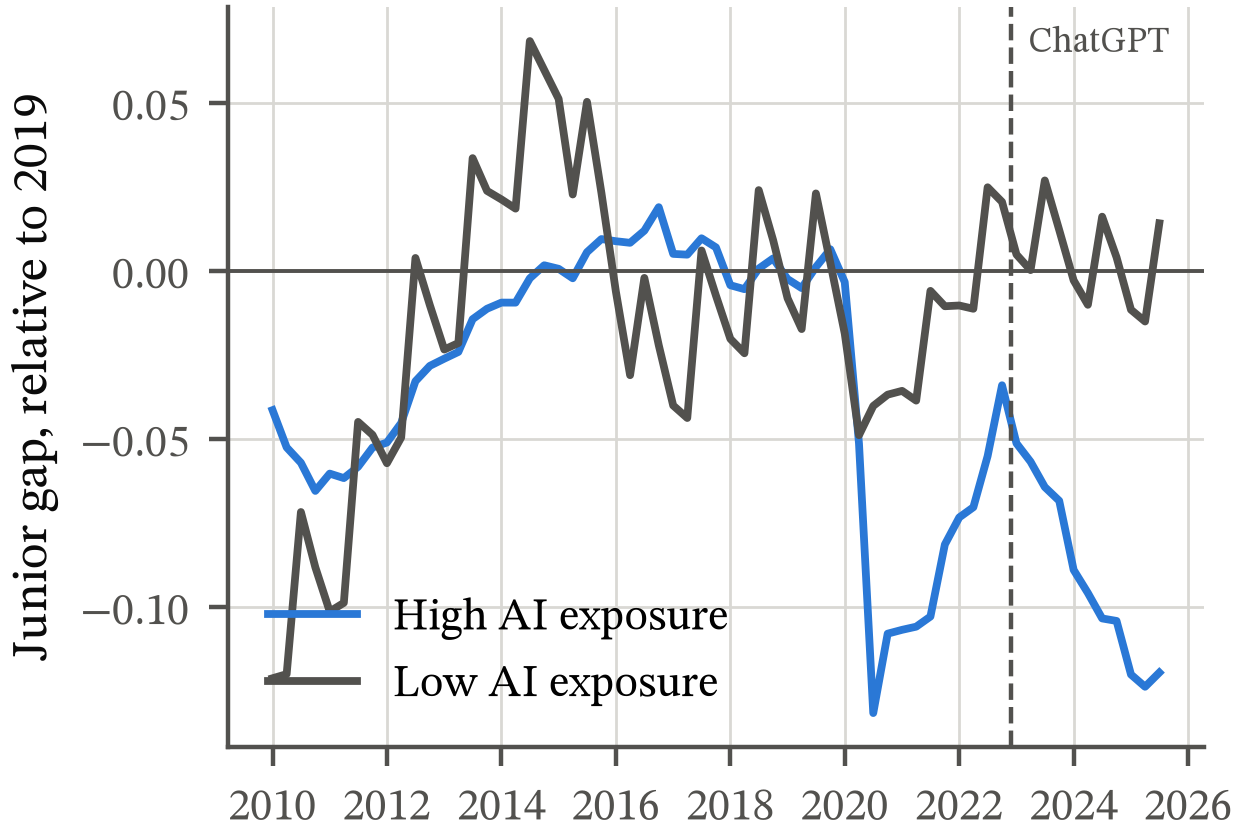
\includegraphics[width=\linewidth]{fig01_junior_gap_by_exposure.png}
    \caption{Junior employment gap}
    \label{fig:raw-junior}
  \end{subfigure}\hfill
  \begin{subfigure}[t]{0.49\textwidth}
    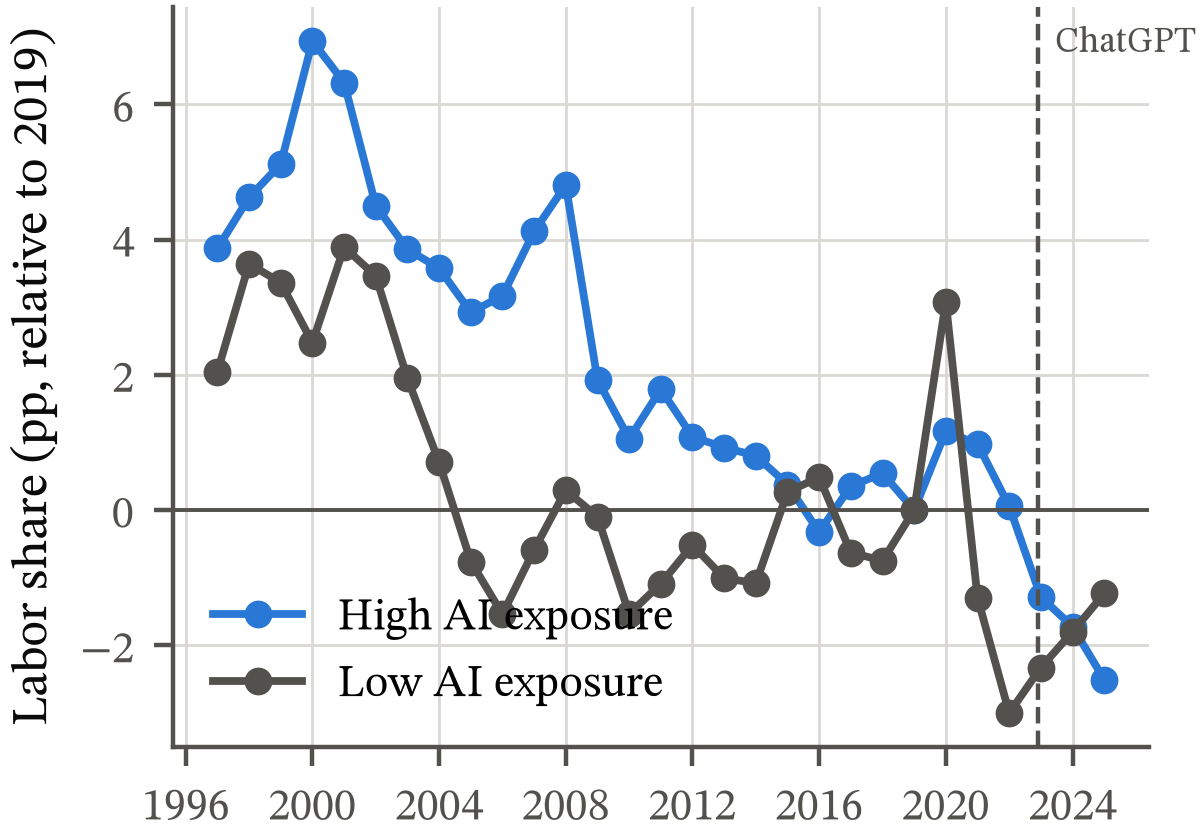
\includegraphics[width=\linewidth]{fig04_labor_share_by_exposure.png}
    \caption{Labor share of value added}
    \label{fig:raw-labor}
  \end{subfigure}
  \caption{Raw data. (a) Log employment of 22--24 year-olds minus log employment of 35--54 year-olds (Census QWI), averaged within the top and bottom thirds of sectors by language-model AI exposure, relative to 2019. (b) Compensation over value added (BEA), averaged within sectors above and below median AI exposure, relative to 2019. These are descriptive; Section~\ref{sec:results} controls for common shocks.}
  \label{fig:raw}
\end{figure}

Figure~\ref{fig:raw} shows the two raw facts that the rest of the paper tests. In high-exposure sectors the junior employment gap collapsed in 2020, recovered through 2022, and has fallen steadily since ChatGPT's release in November 2022; low-exposure sectors show no such pattern. The labor share of high-exposure sectors, which sat above that of low-exposure sectors for most of the last two decades, has fallen below it since 2023. Both pictures are descriptive. A common shock (the 2022--23 rate cycle, for instance) could produce either, and the high-exposure group is dominated by finance and information, whose margins respond to interest rates for reasons that have nothing to do with AI. The empirical design in Section~\ref{sec:data} exists to separate these stories.
